% Original user screenshots; no cropping, redraw, or altered log content.
\begin{center}\begin{minipage}{\linewidth}\centering
\textbf{（a）参考端注错：检测到高位差异并中止}\par\smallskip
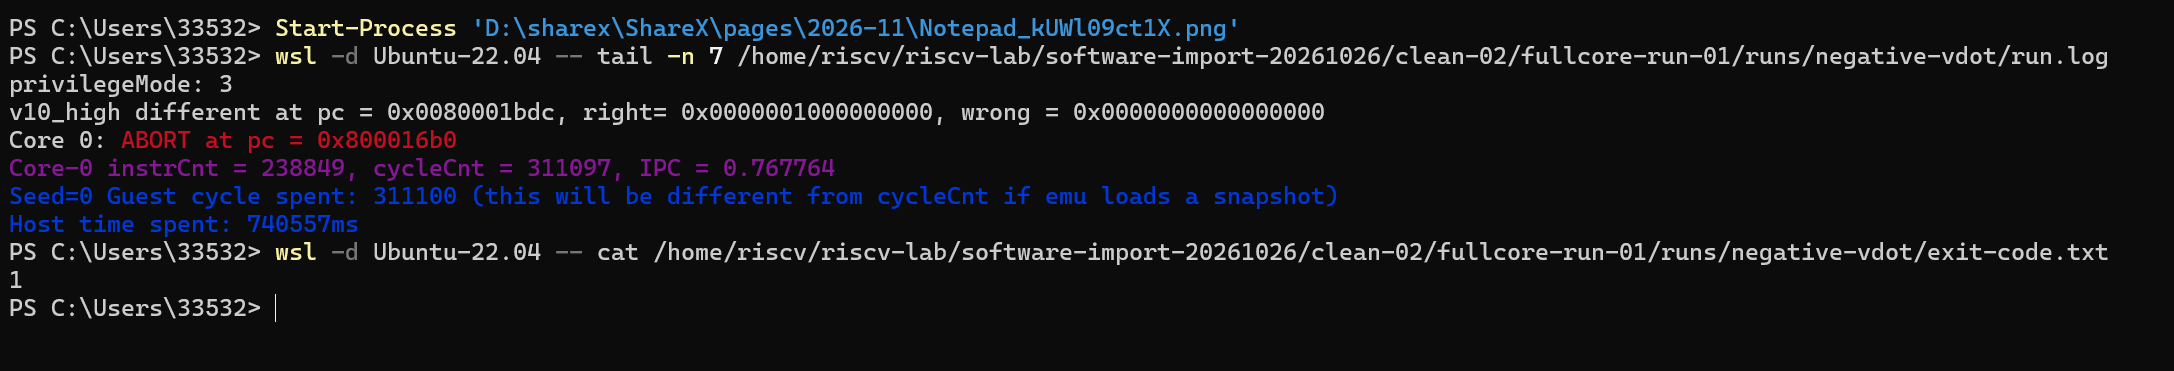
\includegraphics[width=\linewidth]{figures/source-screenshots/S3-03-01-bit100-rejection.png}
\par\medskip
\textbf{（b）正常参考模型：15项通过并正常退出}\par\smallskip
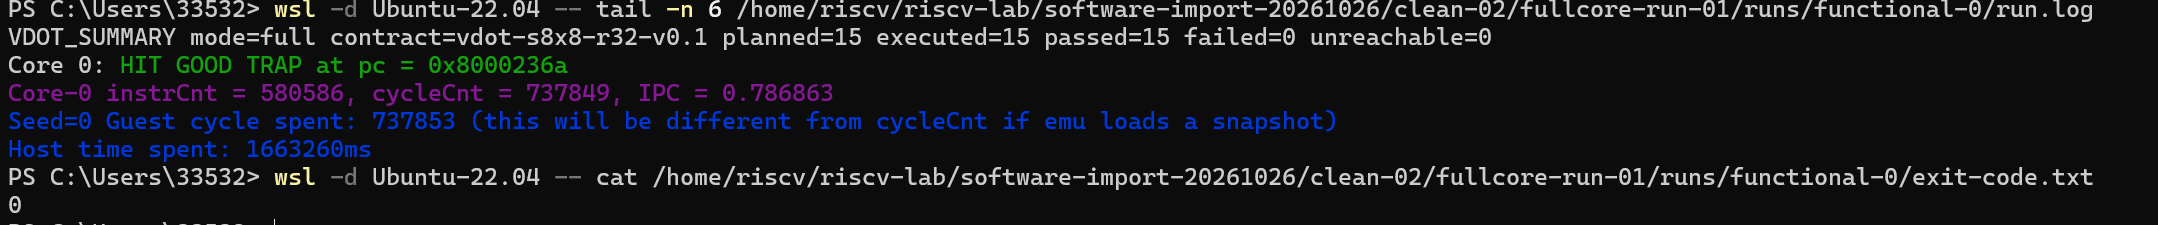
\includegraphics[width=\linewidth]{figures/source-screenshots/S3-03-02-normal-recovery.png}
\captionof{figure}{bit100拒错与正常参考模型恢复验证的原始日志截图}\label{fig:S3-03}
\raggedright\footnotesize
\textbf{注：}上图显示\texttt{v10\_high different}、\texttt{ABORT}及退出码1；差异PC为\texttt{0x80001bdc}，ABORT报告PC为\texttt{0x800016b0}，两者分别保留。参考端故意注错时，\texttt{right/wrong}为比较器两侧标签，不据此判定RTL本身有错。下图显示\texttt{planned=15 executed=15 passed=15 failed=0 unreachable=0}、\texttt{HIT GOOD TRAP}及退出码0。\par
\textbf{来源与范围：}用户提供的历史日志回读截图，来源为\seqsplit{/home/riscv/riscv-lab/software-import-20261026/clean-02/fullcore-run-01/runs/}下\texttt{negative-vdot}与\texttt{functional-0}目录的\texttt{run.log}和\texttt{exit-code.txt}。本次仅补入截图，未重新执行仿真；截图未展示机器字及完整128位结果，相关身份以原始运行记录为准。\par
\end{minipage}\end{center}
